\documentclass[11pt]{article}

\usepackage[margin=1in]{geometry}
\usepackage{amsmath,amssymb}
\usepackage{booktabs}
\usepackage{graphicx}
\usepackage{hyperref}

\newcommand{\linf}{\ell_\infty}

\title{When Weak Features Carry the Attack Surface:\\
A Controlled Study of Feature Reliance and Robustness}
\author{}
\date{}

\begin{document}
\sloppy
\maketitle

\begin{abstract}
A model trained for accuracy uses every feature that helps, including features
that are individually weak. We ask, in a fully known generative task, which
features a trained network uses, how that compares with the statistically
optimal use, and where its adversarial vulnerability sits. The task has one
reliable dimension and five individually weak dimensions that are jointly
informative: the five together reach $96.3\%$ Bayes accuracy, more than the
reliable one alone ($95.5\%$). Four findings. (i)~A trained MLP depends on the
weak channel somewhat \emph{less}, relative to the reliable dimension, than the
Bayes-optimal classifier does (permutation-importance ratio $0.55$ vs.\ $0.72$), so
its vulnerability is not over-reliance on weak features. (ii)~An attacker confined
to the five weak dimensions is $4$--$7\times$ as effective as one confined to the
reliable dimension, but an attacker confined to \emph{one} weak dimension is $3\times$
\emph{less} effective: five coordinates are being compared with one, and only their sum is
dangerous. (iii)~Feature-selective penalties ($L_1$, group Lasso, elastic net) cut
weak-channel attack success from $0.26$ to $0.01$--$0.04$ at $0.96$--$0.98$ accuracy; $L_2$
never reaches that regime, staying above $0.21$ until it collapses. (iv)~The effect
has a recognisable region in parameter space: it vanishes when the reliable feature is
near-perfect, and weight decay is not required to produce it. The mechanism underneath,
the dependence of the flip radius on $\|w\|_1$, is developed in a companion paper; here
we report the empirical structure it must explain.
\end{abstract}

\section{Question and contributions}

Ilyas et al.~\cite{ilyas2019} propose that adversarial examples exploit
\emph{non-robust} features: predictive but brittle. Tsipras et
al.~\cite{tsipras2018} show that using such features can trade accuracy for
robustness. We take the question to a task where everything is known, and ask:
\emph{when a predictor has one reliable feature and several individually weak
but jointly informative ones, which features does gradient-based training use,
how does that compare with the statistically optimal use, and where is the
resulting vulnerability?}

We keep four notions apart that the phrase ``non-robust feature'' tends to
merge. \emph{Predictive reliability} is how well a dimension alone determines
the label (a property of the data). \emph{Joint information} is what several
dimensions carry together. \emph{Learned reliance} is how much the trained
model's decisions depend on a dimension. \emph{Adversarial vulnerability} is how
little perturbation of a dimension flips the output. The first two are fixed by
the generative model before any model is trained, so calling a dimension weak
cannot be circular with finding that it is attackable.

\paragraph{Contributions.}
\begin{enumerate}
\item Weak is not irrelevant: five individually weak dimensions together beat
the reliable one (Section~\ref{sec:bayes}).
\item The trained network under-uses them relative to Bayes. Its vulnerability is
not over-reliance (Section~\ref{sec:bayes}).
\item The vulnerability is carried by the sum of many weak features, not by any one
of them; the usual five-versus-one attack comparison conflates the two
(Section~\ref{sec:attack}).
\item At matched accuracy, only feature-selective regularisation buys robustness
(Section~\ref{sec:reg}).
\item A phase diagram shows where the effect lives and corrects an earlier
attribution to weight decay (Section~\ref{sec:phase}).
\end{enumerate}

Relation to our companion paper~\cite{rootcause}: it derives, for
Gaussian tasks with a linear optimum, that the $\linf$ flip radius is
$|\mathrm{LLR}|/\|w\|_1$ and tests this. This paper reports the empirical
behaviour of trained networks on the same unclipped task. It supersedes our
earlier note~\cite{earlier}, which used clipped inputs; its headline attack
comparison and its claim about weight decay are corrected below, and every
number here was recomputed in the new setting.

\section{Task, models, attacks}
\label{sec:task}

\paragraph{Data.} $x\in\mathbb R^6$ (no clipping), $y\in\{0,1\}$ uniform, and given $y$
the coordinates are independent Gaussians $x_i=(y-\tfrac12)\Delta\mu_i+\sigma_i\xi_i$.
The reliable dimension has $\Delta\mu_0=1$, $\sigma_0=0.3$; the five weak dimensions have
$\Delta\mu=\alpha=0.4$, $\sigma=0.25$. A single threshold on $x_0$ gives $95.2\%$ accuracy
($\Phi(1/0.6)$), on one weak dimension $78.8\%$ ($\Phi(0.4/0.5)$). Without clipping the Bayes
rule is exactly linear, $\mathrm{LLR}=\sum_iw_ix_i$ with $w_i=\Delta\mu_i/\sigma_i^2$
($11.1$ for the reliable dimension, $6.4$ for each weak one). The earlier note clipped to
$[0,1]$, which made $\epsilon=0.5$ reach the boundary from every point; unclipping removes that
artifact.

\paragraph{Models.} One-hidden-layer MLPs (8 ReLU units; Adam, learning rate
$0.02$, 500 steps, weight decay $10^{-2}$; 4{,}000 training and 1{,}000 test
points). \textbf{A}: all six inputs. \textbf{B}: the reliable input only (the weak
dimensions have no input slot). \textbf{C}: six slots with the weak inputs fixed
at $0$, so their weights stay at initialisation.

\paragraph{Attack and uncertainty.} FGSM with an optional coordinate mask
$m$: $x_{\mathrm{adv}}=x+\epsilon\,\mathrm{sign}(\nabla_x\mathrm{CE})\odot m$;
success is the fraction of correctly classified points that flip. We report
$\epsilon\in[0.02,0.3]$. Everything is averaged over 10 seeds (reseeding data and
initialisation) with standard deviations; a multi-step PGD check was run only on the earlier clipped task~\cite{earlier} and
is not repeated here.

\section{What is weak, what is used: the Bayes comparison}
\label{sec:bayes}

Because the generative model is known, the Bayes-optimal rule for any subset of
dimensions can be computed exactly (Monte Carlo, $2\times10^5$ samples).

\begin{table}[h]
\centering
\caption{Accuracy on the test sets of the 10 seeds (mean $\pm$ s.d.): Bayes-optimal rule by input
subset against the trained MLP (Model A).}
\label{tab:bayes}
\begin{tabular}{lc}
\toprule
Classifier & Accuracy \\
\midrule
Bayes, all 6 dimensions & $0.993\pm0.002$ \\
Bayes, $x_0$ only & $0.955\pm0.006$ \\
Bayes, 5 weak dimensions combined & $0.963\pm0.009$ \\
Bayes, 1 weak dimension & $0.789\pm0.009$ \\
\midrule
Trained MLP (Model A) & $0.994\pm0.003$ \\
\bottomrule
\end{tabular}
\end{table}

\textbf{Weak is not irrelevant.} Five conditionally independent, individually
$78.9\%$-accurate dimensions combine to $96.3\%$, above the reliable dimension's
$95.5\%$ (exact values $0.9630$ and $0.9522$ in the earlier clipped task). Their summed
log-likelihood weight is $32.0$ against $11.1$, so a Bayes-optimal classifier places $2.9\times$ more
total weight on the weak channel. (This is a statement about weight $\sum w_i$; in squared
discriminability the ratio is $1.15$.) The weak dimensions are weak only one at a time.

\textbf{The trained network depends on them somewhat less.} Model A's clean accuracy matches
Bayes. To compare reliance on a common footing we use permutation importance: the accuracy drop from
shuffling a channel across the test set and re-applying the unchanged rule.

\begin{table}[h]
\centering
\caption{Permutation-importance accuracy drop, mean $\pm$ s.d.\ over 10 seeds.}
\label{tab:perm}
\begin{tabular}{lccc}
\toprule
Classifier & Reliable permuted & Weak channel permuted & Weak:reliable \\
\midrule
Bayes-optimal & $0.213\pm0.009$ & $0.154\pm0.014$ & $0.72$ \\
Trained MLP (A) & $0.245\pm0.011$ & $0.134\pm0.017$ & $0.55$ \\
\bottomrule
\end{tabular}
\end{table}

The MLP's weak-to-reliable ratio is below the optimum's ($0.55$ vs.\ $0.72$), mostly because it
leans harder on the reliable dimension; its absolute dependence on the weak channel ($0.134$ vs.\
$0.154$) is within about one standard deviation of the optimum's. The effect is therefore real in
direction but modest, and weaker than in the earlier clipped task ($0.36$ vs.\ $0.79$). The
conclusion we draw is limited to this: the MLP's vulnerability is not explained by
over-fitting to weak features, since the weights the optimum places there are already enough. We would not assume this
direction generalises beyond this loss, optimiser and regularisation strength.

\section{Where the vulnerability sits}
\label{sec:attack}

\begin{table}[h]
\centering
\caption{FGSM success at $\epsilon=0.3$, mean $\pm$ s.d.\ over 10 seeds. Clean accuracy: A
$0.994\pm0.003$, B $0.956\pm0.005$, C $0.956\pm0.005$.}
\label{tab:main}
\begin{tabular}{lc}
\toprule
Model / attacked dimensions & Success \\
\midrule
A, all six & $0.536\pm0.020$ \\
A, reliable dimension only & $0.037\pm0.005$ \\
A, five weak dimensions & $0.260\pm0.014$ \\
A, \emph{one} weak dimension & $0.012\pm0.003$ \\
B (reliable input only) & $0.211\pm0.014$ \\
C, all six / weak slots only & $0.211\pm0.014\ /\ 0.000\pm0.000$ \\
\bottomrule
\end{tabular}
\end{table}

\begin{figure}[h]
\centering
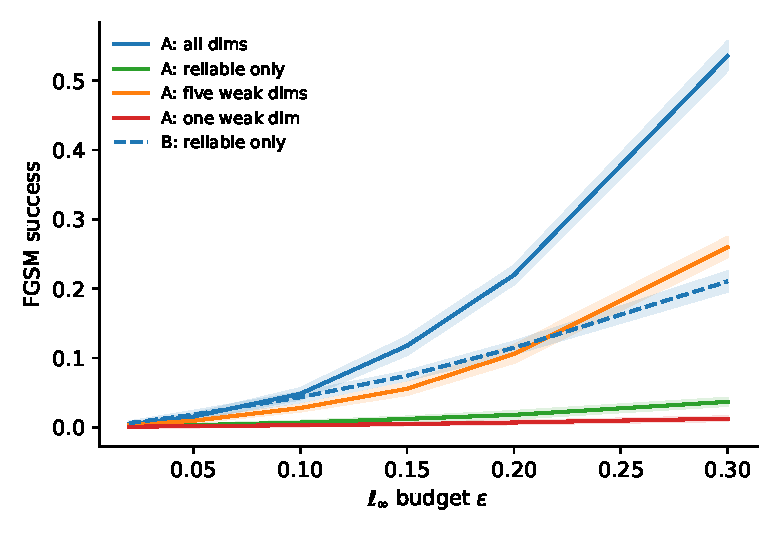
\includegraphics[width=0.62\textwidth]{fig_fr_curves.pdf}
\caption{Attack success against $\linf$ budget for the series of Table~\ref{tab:main}
(mean and $\pm1$ s.d.\ over 10 seeds). One weak dimension (red) is the hardest to exploit;
five together (orange) are far easier than the reliable dimension alone (green).}
\label{fig:curves}
\end{figure}

For budgets of $0.10$ to $0.3$, restricting the attacker to the five weak dimensions is $4$--$7\times$ as effective as
restricting it to the reliable one ($0.260$ vs.\ $0.037$ at $\epsilon=0.3$; $0.028$ vs.\ $0.007$
at $0.10$). Removing the weak dimensions (Model B) cuts full-attack success from $0.536$ to
$0.211$ at a $3.8$-point accuracy cost, and it does so only at larger budgets: for
$\epsilon\le0.10$ the two models are within about a standard deviation ($0.015\pm0.004$ vs.\
$0.018\pm0.005$ at $0.05$, B slightly worse), so the earlier note's ``harder to fool at every
budget from $0.05$'' was too strong. Model C's frozen weak slots are exactly safe at default
initialisation, and stay safe at $10\times$ scale ($0.001\pm0.001$), but become exploitable at
$100\times$ ($0.92\pm0.12$); in a linear model the worst-case logit shift is exactly
$\epsilon\|W_{\mathrm{dead}}\|_1$, which predicts a magnitude threshold of this kind.

\paragraph{The five-versus-one comparison is confounded.} The $4$--$7\times$ figure sets five
attackable coordinates against one, so it mixes \emph{feature type} with \emph{attack
dimensionality}. The control is the row ``one weak dimension'': attacking a single weak dimension
succeeds $0.012$ of the time, $3\times$ \emph{less} than attacking the reliable dimension. Its weight is
smaller ($6.4$ vs.\ $11.1$). The five together are far more exploitable because $\|w_S\|_1$ adds up
($32.0$ vs.\ $11.1$); the companion paper confirms this with exact Bayes flip radii on the same
task ($1.08$ reliable, $1.87$ one weak, $0.37$ five weak)~\cite{rootcause}. So the vulnerability is
not located in any weak feature. Per dimension, weak features are \emph{less} effective to attack;
per attacker, five of them are more effective, simply because there are five. We therefore withdraw the
earlier note's claim that attacks ``through the weak features are more effective'' as a statement
about features, and retain it only as a statement about the number of coordinates the attacker controls.

\section{Which regularisers help}
\label{sec:reg}

Penalties can shrink weights uniformly (\(L_2\)) or select whole input dimensions (first-layer $L_1$,
group Lasso, elastic net). We sweep each strength with 10 seeds and report FGSM success at
$\epsilon=0.3$, with the unpenalised-in-practice baseline (weight decay $10^{-2}$) at $0.994$
accuracy and weak-only success $0.260$. Magnitude pruning of the smallest-norm weak columns
(no retraining) is included for comparison.

\begin{table}[h]
\centering
\caption{Operating points near $0.97$ accuracy, mean $\pm$ s.d.\ over 10 seeds, $\epsilon=0.3$.
Weight ratio is the reliable column norm over the mean weak column norm.}
\label{tab:reg}
\begin{tabular}{lcccc}
\toprule
Method (strength) & Accuracy & Weight ratio & Reliable-only & Weak-only\\
\midrule
Baseline (wd $10^{-2}$) & $0.994\pm0.003$ & $2.0$ & $0.037$ & $0.260\pm0.014$\\
$L_1$ (0.4) & $0.969\pm0.005$ & $18.3$ & $0.173$ & $0.023\pm0.008$\\
Group Lasso (0.4) & $0.975\pm0.005$ & $13.9$ & $0.154$ & $0.038\pm0.012$\\
Elastic net ($L_1{=}0.1$, $L_2{=}0.01$) & $0.979\pm0.004$ & $9.3$ & $0.129$ & $0.050\pm0.008$\\
Elastic net ($L_2{=}0.05$) & $0.963\pm0.006$ & $44.4$ & $0.192$ & $0.011\pm0.006$\\
Pruning, no retrain ($k{=}4$) & $0.970\pm0.005$ & $9.1$ & $0.139$ & $0.052\pm0.007$\\
$L_2$ (0.2) & $0.993\pm0.003$ & $2.3$ & $0.044$ & $0.213\pm0.013$\\
$L_2$ ($\ge0.4$) & $0.488\pm0.011$ & -- & -- & --\\
\bottomrule
\end{tabular}
\end{table}

Feature-selective penalties move to an operating point where weight sits on the reliable
dimension and weak-only success falls by an order of magnitude ($0.26\to0.01$--$0.04$) for $1.5$--$3$ points of accuracy.
$L_2$ cannot get there: with strength up to $0.2$ it costs no accuracy and lowers weak-only success only
modestly ($0.260\to0.213$), and at $0.4$ it collapses to chance, with nothing in between. So at the same accuracy
cost there is no $L_2$ counterpart to compare with; the comparison is between a tunable frontier
and a cliff. Pruning without retraining traces a smooth frontier too, but a worse one: at $0.970$ accuracy it leaves
weak-only success at $0.052$, twice $L_1$'s $0.023$ at the same accuracy. This is the earlier trade at work: selective
penalties buy robustness by discarding evidence, and the accuracy they give up is the information the weak channel carried;
the companion paper shows the same exchange on the task with an $L_1$ sweep~\cite{rootcause}. We did not test pruning with
fine-tuning, or selective penalties on real data.

\section{Where the effect lives: a phase diagram}
\label{sec:phase}

We retrain Model A on a grid of $\sigma_0\in\{0.1,\ldots,0.5\}$ (reliable-dimension noise),
$\alpha\in\{0.1,0.2,0.4,0.6\}$ (weak-feature strength) and weight decay
$\in\{0,10^{-3},10^{-2},10^{-1}\}$, 5 seeds per cell, and measure FGSM success at
$\epsilon=0.2$ restricted to the weak dimensions.

\begin{figure}[h]
\centering
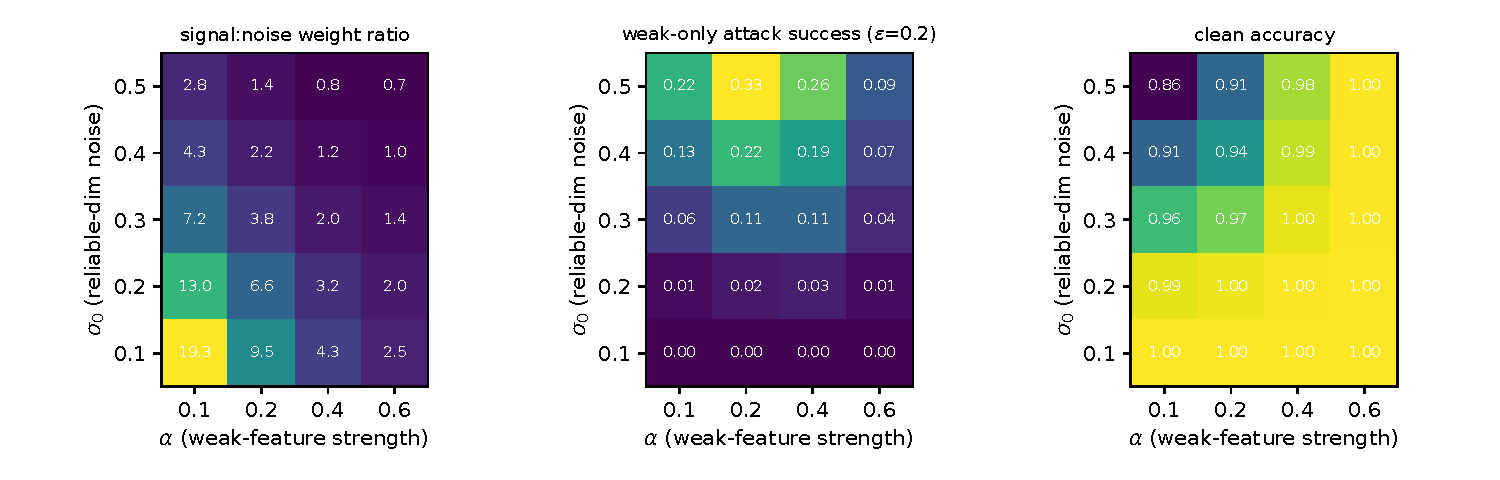
\includegraphics[width=\textwidth]{fig_fr_phase.pdf}
\caption{Phase diagram at weight decay $10^{-2}$, 5 seeds per cell. Left: reliable:weak weight
ratio. Middle: weak-dimension-only attack success at $\epsilon=0.2$. Right: clean accuracy.}
\label{fig:phase}
\end{figure}

Three observations. (a)~\emph{Onset.} At $\sigma_0=0.1$ (near-deterministic reliable
feature) weak-only success is $\le0.001$ everywhere on the grid. With a near-perfect reliable feature,
cross-entropy saturates and the weak channel is left unused. This is a statement about optimisation, not about the
weak features being uninformative: Section~\ref{sec:bayes} shows they carry substantial information.
(b)~\emph{Growth.} Weak-only success grows with $\sigma_0$ and peaks at $\alpha=0.2$--$0.4$, reaching $0.37$ at
$\sigma_0=0.5$, $\alpha=0.2$ with no weight decay (against $0.11$ at the main operating point $\sigma_0=0.3,\alpha=0.4$
with $\epsilon=0.2$, weight decay $10^{-2}$). For $\sigma_0\ge0.4$ and strong weak features
($\alpha\ge0.4$) the weight ratio falls to $0.67$--$1.2$, i.e.\ the model relies about as much per dimension on a weak
feature as on the reliable one; we did not characterise this regime further. (c)~\emph{Weight decay is not the cause.}
The earlier note attributed the effect to an imperfect signal \emph{and} weight decay. Sweeping them independently shows
an imperfect signal alone suffices, and that at fixed $(\sigma_0,\alpha)$ increasing weight decay
\emph{reduces} weak-channel reliance, monotonically in both rows we checked ($0.122\to0.116\to0.110\to0.095$ at
$\sigma_0=0.3,\alpha=0.4$; $0.248\to0.244\to0.217\to0.105$ at $\sigma_0=0.5,\alpha=0.1$). This corrects the earlier attribution.

\section{Discussion}

\paragraph{What the controlled setting buys.} Because reliability and joint information are fixed
by the generative process, four questions can be separated that the phrase ``non-robust
features'' runs together: weak (data), jointly informative (data), used (model), vulnerable (attack).
The answers here are that weak features are not irrelevant, the model uses them somewhat less than
the optimum does, the vulnerability is a property of their sum, and the benefit of removing them is paid for
in accuracy.

\paragraph{Mechanism.} The attacker's budget is spent across all coordinates the model reads, so a
linear score moves by $\epsilon\|w\|_1$ and the flip radius is $|\mathrm{LLR}|/\|w\|_1$; five modest weights
add to $32.0$ against $11.1$. This is why a coalition of weak features is easy to move while each
member alone is hard, and why selective regularisation (which shrinks $\|w\|_1$) helps where $L_2$
(which shrinks all weights toward the same ratio) does not at matched accuracy. The derivation and the
spread-versus-scale decomposition are in~\cite{rootcause}.

\paragraph{Activation sparsity.} An activation penalty $\lambda\bar h$ lowers hidden activity as
intended but has no handle on individual input dimensions, and individual seeds fall from
functional to dead networks at different $\lambda$ (so the mean degrades smoothly only as an
averaging artifact)~\cite{earlier}. Weight sparsity has a feature-selection axis; activation sparsity
does not. We report this as a methodological caution on averaging over seeds, not as a mechanism claim.

\paragraph{Limitations.} One task family, equal-weight independent features, a single small
architecture, and FGSM only in this paper (a PGD check exists only for the earlier clipped task, and minimal-radius
attacks are in~\cite{rootcause}).
We did not test correlated weak features, deeper networks or real data. The $L_1$ and group-Lasso gains
depend on feature columns being the right unit of selection, which is a design property of this task.
A circle-versus-square image analogue in~\cite{earlier} reproduces vulnerability through the
background cue but cannot separate region from channel; we treat it as secondary evidence and do not
repeat it.

\section{Conclusion}

In a task where everything is known, a trained network is vulnerable through a channel of individually
weak but jointly informative features that it actually uses \emph{less} than the Bayes-optimal
classifier would. The vulnerability belongs to the channel as a whole rather than to any single
feature, it is removable by feature-selective regularisation at the price of the information those
features carry (a trade that $L_2$ cannot make smoothly), and it occupies a recognisable region of the parameter space of reliable-feature noise and weak-feature
strength, independent of weight decay. A model reading all of them is more accurate and less robust; the exchange rate is the information those features carry.

\begin{thebibliography}{9}

\bibitem{rootcause}
Companion paper: \emph{Where Does Adversarial Vulnerability Come From? A Controlled Gaussian
Study with a Real-Data Check} (\texttt{root\_cause\_paper.tex}, this repository).

\bibitem{earlier}
Earlier note: \emph{Robust and Non-Robust Features in a Fully Controlled Synthetic Classification
Task: A Minimal Demonstration} (\texttt{toy\_robust\_features\_paper.tex}, this repository).

\bibitem{ilyas2019}
A.~Ilyas, S.~Santurkar, D.~Tsipras, L.~Engstrom, B.~Tran, A.~Madry.
\emph{Adversarial Examples Are Not Bugs, They Are Features}. NeurIPS, 2019.

\bibitem{tsipras2018}
D.~Tsipras, S.~Santurkar, L.~Engstrom, A.~Turner, A.~Madry.
\emph{Robustness May Be at Odds with Accuracy}. ICLR, 2019.

\end{thebibliography}

\end{document}
